\section{Introduction}
\label{sec:clio:introduction}

Modern datacenter applications like graph computing, data analytics, and deep learning have an increasing demand for access to large amounts of memory~\cite{FastSwap}.
Unfortunately, servers are facing {\em memory capacity walls} because of pin, space, and power limitations~\cite{HP-MemoryEvol,ITRS14,MemoryWall95}.
Going forward, it is imperative for datacenters to seek solutions that can go beyond what a (local) machine can offer, \ie, using remote memory.
At the same time, datacenters are seeing the needs from management and resource utilization perspectives
to {\em disaggregate} resources~\cite{Ali-SinglesDay,SnowFlake-NSDI20,FB1}\textemdash separating hardware resources into different network-attached pools 
that can be scaled and managed independently.
These real needs have pushed the idea of memory disaggregation ({\em \md} for short):
organizing computation and memory resources as two separate network-attached
pools, one with compute nodes ({\em CN}s) and one with memory nodes ({\em MN}s).

So far, \md\ researches have all taken one of two approaches: 
building/emulating \MN{}s using regular servers~\cite{AIFM,InfiniSwap,FastSwap,Shan18-OSDI,zombieland} 
or using raw memory devices with no processing power~\cite{Tsai20-ATC,Lim09-disaggregate,Lim12-HPCA,HP-TheMachine}.
%,ATC21Paper
%\textit{Is it possible to build \MN{}s without a server}, as promised by the original proposal of \md~\cite{Lim09-disaggregate,Shan18-OSDI}?
The fundamental issues of server-based approaches such as RDMA-based systems are the monetary and energy cost of a host server and the inherent performance and scalability limitations caused by the way NICs interact with the host server's virtual memory system.
Raw-device-based solutions have low costs.
However, they introduce performance, security, and management problems
because when \MN{}s have no processing power, all the data and control planes have to be handled at \CN{}s~\cite{Tsai20-ATC}.
%\MN{}s become too ``dumb'' and low level when removing its processing power altogether.
%overhead of root cause why RDMA is unfit for \md\ is that it is designed to work around a host server,
%and traditional servers' virtual memory system is not designed for \md.
%Contrary to server-based \md\ solutions, \pdm\ is another extreme where there is no processing at all at \MN{}s.
%The root cause of \pdm's various performance, security, and management problems is exactly this: 
%\MN{}s are too ``dumb'' and low level.

%From the above discussion, we find that both server-based \md\ and raw physical \md\ have their limitations.
Server-based \MN{}s and \MN{}s with no processing power are two extreme approaches of building \MN{}s.
We seek a sweet spot in the middle by proposing a hardware-based \md\ solution that has the right amount of processing power at \MN{}s.
%for the right type of \MN{} management system.
%To mitigate RDMA's various issues for \md, one could try to improve RDMA's hardware design or add a software layer to work around RDMA's problems.
%This paper takes a different approach by starting
Furthermore, we take a clean-slate approach by starting from the requirements of \md\
and designing a \md-native system.
%LegoOS is the only existing work that also proposes a .
%Unfortunately, LegoOS still uses server software and the RDMA network to emulate its hardware design, leaving all the research questions we ask in this paper unanswered.


We built {\em \sys}\footnote{Clio is the daughter of Mnemosyne, the Greek goddess of memory.}, a hardware-based disaggregated memory system.
%focusing on the hardware-based virtual memory system and network stack.
\sys\ includes a \CN-side user-space library called {\em \syslib}
and a new hardware-based \MN\ device called {\em \sysboard}.
Multiple application processes running on different \CN{}s can allocate memory from the same \sysboard, with each process having its own {\em remote virtual memory address space}.
Furthermore, one remote virtual memory address space can span multiple \sysboard{}s.
Applications can perform byte-granularity remote memory read/write and use \sys's synchronization primitives for synchronizing concurrent accesses to shared remote memory .

A key research question in designing \sys\ is \textit{\textbf{how to use limited hardware resources to achieve 100\Gbps, microsecond-level average and tail latency for TBs of memory and thousands of concurrent clients?}}
These goals are important and unique for \md.
A good \md\ solution should reduce the total CapEx and OpEx costs compared to traditional non-disaggregated systems and thus cannot afford to use large amounts of hardware resources at \MN{}s.
Meanwhile, remote memory accesses should have high throughput and low average and tail latency, because even after caching data at \CN-local memory, there can still be fairly frequent accesses to \MN{}s and the overall application performance can be impacted if they are slow~\cite{disagg-osdi16}.
Finally, unlike traditional single-server memory, a disaggregated \MN\ should allow many \CN{}s to store large amounts of data so that we only need a few of them to reduce costs and connection points in a cluster.
%cost, performance, and scalability goals 
How to achieve each of the above cost, performance, and scalability goals {\em individually} is relatively well understood.
%: using hardware to achieve high performance, using more hardware to support larger scales, and using fewer hardware to reduce costs.
However, achieving all these seemingly conflicting goals {\em simultaneously} is hard and previously unexplored.

Our main idea is to \textbf{\textit{eliminate state from the \MN\ hardware}}.
Here, we overload the term ``state elimination'' with two meanings: 1) the \MN\ can treat each of its incoming requests in isolation even if requests that the client issues can sometimes be inter-dependent, 
and 2) the \MN\ hardware does not store metadata or deals with it.
Without remembering previous requests or storing metadata, an \MN\ would only need a tiny amount of on-chip memory that does not grow with more clients, thereby {\em saving monetary and energy cost} and achieving {\em great scalability}.
Moreover, without state, the hardware pipeline can be made {\em smooth} and {\em performance deterministic}.
A smooth pipeline means that the pipeline does not stall, which is only possible if requests do not need to wait for each other.
It can then take one incoming data unit from the network every fixed number of cycles (1 cycle in our implementation), achieving constantly {\em high throughput}.
A performance-deterministic pipeline means that the hardware processing does not need to wait for any slower metadata operations and thus has {\em bounded tail latency}.
%When and only when complete elimination is impossible, we . 

Effective as it is, can we really eliminate state from \MN\ hardware? 
First, as with any memory systems, users of a disaggregate memory system expect it to deliver certain reliability and consistency guarantees (\eg, a successful write should have all its data written to remote memory, a read should not see the intermediate state of a write, etc.). 
Implementing these guarantees requires proper ordering among requests and involves state even on a single server. 
The network separation of disaggregated memory would only make matters more complicated.
Second, quite a few memory operations involve metadata, and they too need to be supported by disaggregated memory.
Finally, many memory and network functionalities are traditionally associated with a client process and involve per-process/client metadata (\eg, one page table per process, one connection per client, etc.). 
Overcoming these challenges require the re-design of traditional memory and network systems.
%How can we overcome these challenges to eliminate state from \MN\ hardware?
%The network separation of \MN{}s and \CN{}s means that packets could potentially be dropped or reordered. 
%Traditional 
%\textbf{\textit{How can we eliminate state from \MN\ hardware when remote memory operations are stateful by nature?}}
%For example, memory allocation needs to check the state of space availability; reliable memory operations over the network requires state for ordering and re-transmission.

Our first approach is to separate the metadata/control plane and the data plane, with the former running as software on a low-power ARM-based SoC at \MN\ and the latter in hardware at \MN. 
Metadata operations like memory allocation usually need more memory but are rarer (thus not as performance critical) compared to data operations.
A low-power SoC's computation speed and its local DRAM are sufficient for metadata operations.
On the other hand, data operations (\ie, all memory accesses) should be fast and are best handled purely in hardware. 
Even though the separation of data and control plane is a common technique that has been applied in many areas~\cite{4d-sdn,netvirt,arrakis}, a separation of memory system control and data planes has not been explored before and is not easy, as we will show in this paper.

Our second approach is to re-design the memory and networking data plane so that most state can be managed only at the \CN\ side.
Our observation here is that the \MN{} only {\em responds} to memory requests but never {\em initiates} any.
This \CN-request-\MN-respond model allows us to use a custom, connection-less reliable transport protocol that implements almost all transport-layer services and state at \CN{}s, allowing \MN{}s to be free from traditional transport-layer processing.
%optimized for transferring memory requests and responses between CNs and MNs, which is much simpler and more scalable than RDMA, thanks to its stateless operation at MNs.  
Specifically, our transport protocol manages request IDs, transport logic, retransmission buffer, congestion, and incast control all at \CN{}s. It provides 
reliability by ordering and retrying an entire memory request at the \CN\ side.
%This \CN-request-\MN-respond model allows us to use a connection-less, RPC-based network protocol between \CN\ and \MN\ and build the \MN\ with only the physical and link network layers (\ie, no transport layer or above).
%a ``transport-less'' \MN\ network design.
%We then manage request IDs, transport logic, retransmission buffer, congestion and incast control all at \CN{}s.
%Furthermore, we provide reliability by ordering and retrying an entire memory request at the \CN\ side.
As a result, the \MN{} does not need to worry about per-request state or inter-request ordering and only needs a tiny amount of hardware resources which do not grow with the number of clients.
 
With the above two approaches, the hardware can be largely simplified and thus cheaper, faster, and more scalable.
However, we found that \textit{\textbf{complete state elimination at \MN{}s is neither feasible nor ideal}}. To ensure correctness, the \MN\ has to maintain some state (\eg, to deal with non-idempotent operations). To ensure good data-plane performance, not every operation that involves state should be moved to the low-power SoC or to \CN{}s.
Thus, our approach is to eliminate as much state as we can without affecting performance or correctness and to carefully design the remaining state so that it causes small and bounded space and performance overhead.

For example, we perform paging-based virtual-to-physical memory address mapping and access permission checking at the \MN\ hardware pipeline, as these operations are needed for every data access.
Page table is a kind of state that could potentially cause performance and scalability issues but has to be accessed in the data path.
We propose a new overflow-free, hash-based page table design where 1) all page table lookups have bounded and low latency (at most one DRAM access time in our implementation), and 2) the total size of all page table entries does not grow with the number of client processes.
As a result, even though we cannot eliminate page table from the \MN\ hardware, we can still meet our cost, performance, or scalability requirements.

Another data-plane operation that involves metadata is page fault handling, which is a relatively common operation because we allocate physical memory on demand.
Today's page fault handling process is slow and involves metadata for physical memory allocation.
We propose a new mechanism to handle page faults in hardware and finish all the handling within bounded hardware cycles.
We make page fault handling performance deterministic by moving  physical memory allocation operations to software running at the SoC.
We further move these allocation operations off the performance-critical path by pre-generating free physical pages to a fix-sized buffer that the hardware pipeline can pull when handling page faults.

We prototyped \sysboard\ with a small set of Xilinx ZCU106 MPSoC FPGA boards~\cite{ZCU106} and built three applications using \sys:
a FaaS-style image compression utility, a radix-tree index, and a key-value store.
%We prototyped \sys's memory device with FPGA (\sysboard).
%\sys\ achieves high throughput (100\Gbps\ with FPGA prototype), low (tail) latency (XXX\mus\ end-to-end MTU round trip latency), 
%low cost (XXX\x\ energy saving), %and great extendibility,
%and \sys\ scales well with XXX. %eliminates {\em all} scalability bottlenecks in both its memory and network systems.
We compared \sys\ with native RDMA, two RDMA-based disaggregated/remote memory systems~\cite{Tsai20-ATC,Kalia14-RDMAKV}, 
a software emulation of hardware-based disaggregated memory~\cite{Shan18-OSDI},
%an FPGA-based RDMA implementation~\cite{StRoM}, 
and a software-based SmartNIC~\cite{BlueField}.
\sys\ scales much better and has orders of magnitude lower tail latency than RDMA, 
while achieving similar throughput and median latency as RDMA (even with the slower FPGA frequency in our prototype).
\sys\ has 1.1\x\ to 3.4\x\ energy saving compared to CPU-based and SmartNIC-based disaggregated memory systems 
and is 2.7\x\ faster than SmartNIC solutions. 
%From our efforts of building \sys, we found that complete state elimination at \MN{}s is neither feasible nor necessary. Instead, we eliminate as much state as we can without affecting performance or correctness and carefully design the remaining state so that it causes small and bounded space and performance overhead.
\sys\ is publicly available at \url{https://github.com/WukLab/Clio}.
%We will make \sys\ publicly available upon this paper's publication.



\if 0
A \sysboard\ consists of three main components: 1) a hardware chip that integrates a thin network stack and a virtual memory system to handle data requests (the {\em fast path}), 2) an ARM processor that runs software to handle metadata requests and background tasks (the {\em slow path}), and 3) an FPGA that hosts application computation offloading (the {\em extend path}).

In building \sys, we explore new requirements, challenges, and benefits of \md.
Specifically, we answer three important research questions.

First, \textbf{how does the design and implementation of a
dedicated hardware \MN\ differ from server and programmable NIC
designs?}
%To protect the accesses from different applications to the memory in an \MN\ and to make such accesses flexible, 
%we should use a virtual memory system to check and map virtual memory addresses to physical addresses.
Current \md\ solutions rely on a host server (its OS and MMU) to provide a virtual memory system so that accesses to the memory are protected and flexible. 
Using a whole server just for the virtual memory system is overkill and unnecessarily adds monetary and energy costs to \md. %consumes too much power.
Another possibility is to use a low-power processor (\eg, ARM) in a SmartNIC to run the virtual memory system~\cite{iPipe}. 
However, doing so has high performance impact mainly because the virtual memory system is on a separate chip from the NIC.
%However, doing so has performance overhead, both because the virtual memory system is on a separate chip from the NIC
%and because the virtual memory system is not designed for \md.
%To date, there has been no attempt
%\yizhou{I think here we should emphasize that: MNs emulated using host server has cost and power waste while the SmartNIC-based ones have perf issue. In all, there is no ideal solution for building real server-less MNs. Hence we took a ...}
Overall, server-based approaches have cost overheads while SmartNIC solutions have performance overheads.
We took a clean-slate approach by building a hardware-based virtual memory system that is integrated with a customized hardware network stack, 
both of which are designed specifically for handling virtual memory requests sent over the network.

Second, \textbf{how can a low-cost \MN\ host TBs of memory and support thousands of concurrent application processes?}
Different from traditional (local) memory, an \MN\ is intended to be shared by many applications running at different \CN{}s,
and the more applications it can support, the more efficiently its memory can be utilized.
Thus, we aim to have each \MN\ host TBs of memory for thousands of concurrent applications processes.
However, a hardware design is constrained by the limited resources in a hardware chip such as on-chip memory.
Compared to traditional software-based virtual memory systems, 
how can an \MN\ use orders of magnitude less resources while achieving orders of magnitude higher scalability?
%which raises the problem of how to manage the scalability we target in hardware.
%is especially accute in an \hdm\ because of its low cost requirements.
Current solutions like RDMA NICs swap metadata between NIC's on-chip memory and host server memory,
which comes with performance overhead (4\x\ compared with when metadata is in the NIC memory~\cite{Pythia}).
%RDMA improves scalability by adding more hardware resources to cache more metadata/states), which comes with increasing monetary and energy costs.

Our clean-slate approach is to carefully examine each virtual-memory and networking task 
and to redesign them to 1) eliminate states and metadata whenever possible (\eg, by minimizing indirection),
2) move complex but non-performance-critical states, metadata, and tasks to the software slow path,
3) shift functionalities to the \CN\ (\syslib) to reduce \MN's complexity 
(\eg, our network transport runs at \syslib, and \MN\ is ``transport-less''),
and 4) design bounded-size, inherently scalable data structures.
%For the remaining functionalities that still need caching, we redesign them to guarantee good cache-miss performance.
As a result, each \MN\ (\sysboard) could support TBs of memory and thousands of application processes with only 1.5\MB\ on-chip memory.
%\yizhou{On top of network scalability, I think its also worth explaining how we are able to support TBs of memory. Because this reminds me of O(1) memory issues. With TBs of memory, the memory related metadata and OPs increased as well. Our pros: our fast path use huge page + hashtable-based pgtable, bounded latency. Our cons: our buddy allocator running in ARM is still prone to this huge memory issue.}
%For certain functionalities, we avoid states and metadata alltogether by re-designing the functionalities.
%For functionalities that could be and move the ones that can be moved to the \CN\ side.
%and not relying on cache for good performance.

Third, \textbf{how to minimize tail latency in a \md\ system}?
%\textbf{is it possible to minimize tail latency by processing all read/write requests deterministically?} 
Tail latency is important in datacenters especially for workloads that have large fanouts (\eg, Spark jobs).
Although much effort has focused on improving the network and core scheduling for low tail latency~\cite{nanoPU,Shenango,Shinjuku,ZygOS,RPCValet},
the memory system has largely been overlooked.
However, the (remote) memory system is what contributes to extreme long tails in a \md\ system.
For example, RDMA's round-trip latency is around 1--2\mus\ in the common case,
but its tail could be as long as 16.8\ms\ (Figure~\ref{fig-miss-hit} and \S\ref{sec:clio:rdma}). % (when there is a page fault).
%The main reason for RDMA's various tails is its reliance on the host virtual memory system, which is not designed for \md\ or for low tail latency.

We reexamine traditional memory system
%from the tail latency and perspectives 
and propose a set of novel mechanisms to bound \sys's tail latency.
Our core idea is to include {\em all} the functionalities that are needed to fulfill all types of data requests in one hardware pipeline
and to make this hardware pipeline {\em performance deterministic}.
This pipeline takes one incoming data unit every cycle (\ie, no pipeline stalls) and completes every request in a fixed number of cycles,
which yields 100\Gbps\ throughput, 2.5\mus\ at median and 3.2\mus\ at 99-percentile end-to-end latency (Figure~\ref{fig-tail-latency}).
Two major technical hurdles in achieving this performance are to perform page table lookups and to handle page faults in a bounded, short time period.  
For the former, we propose a new {\em overflow-free} hash-based page table that bounds all page table lookups to {\em at most one DRAM access} (instead of the long page table walk in a traditional CPU architecture).
For the latter, we propose a new mechanism to handle page faults in hardware with bounded cycles (instead of the costly process of interrupting and handling page faults in the OS).

\fi

%These mechanisms include 1) handling page faults in hardware,
%2) d
%RDMA’s way is to pre-reserve memory and to use large on-device cache. But cache can’t always work, and reserving memory results in inefficient memory utilization.
%Our solution is to allocate physical memory on-demand and to make the cache miss path fast by handling page faults in hardware and by designing a new hash-based page table. We also carefully designed our hardware pipeline to have deterministic, bounded latency.




\if 0
%Unlike traditional computer
%modern computers that manage and use memory at the same place,
% where memory is managed and used at the same place, % at the server CPU and MMU,
Unlike traditional computers that manage and use memory at the same place,
there are many ways of building a disaggregated memory system when memory is far from computation.
For example, should memory be managed at \CN{}s or \MN{}s?
Should \MN{}s be full server boxes, raw DRAM chips, or something in between?
Should computation only happen at \CN{}s or can some of it happen at \MN{}s as well?

Memory disaggregation also poses new requirements in performance, scalability, cost, and deployment.
Like today's storage disaggregation solutions~\cite{AMAZON-S3,SnowFlake-NSDI20,Pangu}, 
the disaggregated memory pool is intended to host large amounts of memory
that can be shared by many clients.
At the same time, to be an appealing solution that can be adopted by today's datacenters, 
memory disaggregation should improve performance per dollar and be easy to deploy and manage.
%and have an easy way 
%At the same time, it is desirable to maintain or decrease data-center costs
%when introducing memory disaggregation.
%Thus, each \MN\ 
%Memory disaggregation presents new requirements in performance, cost
%Existing approaches in building disaggregated-memory systems take three main forms,
%and they have different choices of the above questions and their own limitations.

Existing memory disaggregation solutions have taken two main approaches,
neither of which can meet all the above requirements.
The first type treats \MN{}s as raw, physical memory 
and manage it at \CN{}s~\cite{Genz-citation,CXL-citation,Tsai20-ATC}.
Although \MN{}s are cheap to build, using and managing them at \CN{}s
is slow because of the network round trips needed to access \MN{}s.
%which causes high communication overhead and security concerns, 

The second type accesses \MN{}s over a virtual memory interface
and relies on a host server to virtualize and manage memory at \MN{}s. 
RDMA-based solutions~\cite{FaRM,FastSwap,InfiniSwap,StRoM,Kalia14-RDMAKV,Aguilera18-ATC} all fall into this category.
%The main issue with this approach is the involvement of host 
Using a whole server to manage memory is overkill and unnecessarily consumes too much power.
Moreover, with today's server architecture, a NIC needs to either suffer from a slow crossover to the host memory and/or CPU for 
fetching virtual memory metadata and executing virtual memory tasks like page fault handling~\cite{NICPageFaultArchPaper},
or use limited on-NIC memory to cache metadata, which results in serious scalability issues~\cite{FaRM,Tsai17-SOSP}.
%or rely on a host server to run a virtual memory system (RDMA- and messaging-based),
%which has tail latency, scalability, and cost issues.

We argue that memory disaggregation can and should achieve all the performance, scalability, cost, and deployment requirements.
The solution is to virtualize and manage disaggregated memory in hardware and build \MN\ as a stand-alone device,
as doing so avoids the energy cost of a power-hungry server CPU and the performance overhead to cross multiple devices in a server.
%can achieve better scalability and performance with hardware pipelining and parallelism.
We propose \textit{\sys} (\textit{Disaggregated Virtual Memory Access}), 
a cross-layer, software/hardware-codesign solution that %centers around 
%allows both applications running at \CN{}s and computation offloads running at \MN\ hardware
allows applications to access disaggregated memory through a virtual memory interface
and at the same time, allows \MN{}s to be built without a server box.
%\sys\ includes a memory system, a network system, and a framework for computation offloading,
%all of which are catered towards the hardware-based disaggregated virtual memory model and memory disaggregation's unique requirements.
The \sys\ \MN\ is a new hardware device (\textit{\sysboard}) that we designed from scratch and prototyped with FPGA. %a Xilinx FPGA-based MPSoC board.
The rest of \sys\ uses common hardware and network infrastructure available in today's datacenters with a user-space library (\textit{\syslib}) at each \CN,
making \sys\ easy to be adopted.
The key piece of \sys\ is a hardware-based virtual memory system that runs entirely in \sysboard.
It achieves the same functionality as traditional, software-based virtual memory system,
but with very different approaches --- new designs that fit the hardware model and memory disaggregation.
\sys\ also includes a new network system that we co-design with \sys's memory system
by exploiting memory disaggregation's {\em asymmetric} nature.
Finally, to mitigate the network communication costs between \CN{}s and \MN{}s,
\sys\ creates a framework for applications to safely and easily offload their computation.
% support computation offloading (from \CN{}s to \MN{}s),
%both catered towards the hardware-based virtual disaggregated memory model.

\sys\ offers three ways of using disaggregated memory.
First, applications or a system layer (\eg, a swap system~\cite{InfiniSwap,FastSwap}) running at \CN{}s can allocate (remote) virtual memory spaces and read/write data in them.
In addition, \sys\ offers a set of extended APIs like synchronization primitives and pointer chasing, % for applications running at \CN{}s to use,
and users can also write and deploy new extended APIs at \MN{}s.
Second, applications can offload some of their computation to \MN{}s.
\sys\ provides such offloads with the same virtual memory address space and interface as their \CN\ counterparts.
Finally, users can build \textit{memory services} that run entirely at \MN{} hardware (\eg, a key-value store).
\sys\ offers each memory service its own virtual memory address space.

\sys\ achieves 
\textbf{1) \textit{low tail latency and high throughput}} --- \sys\ achieves network line rate (100\Gbps\ with our FPGA prototype)
and low average and tail latency (\eg, 2.7\mus\ avg and 3.2\mus\ 99-percentile for 1000 clients concurrently reading 16\,B), 
\textbf{2) \textit{excellent scalability}} --- one \MN{} can %freely\footnote{as long as sustainable by port link bandwidth and total memory size}
scale perfectly to thousands of concurrent clients and TBs of memory, % with the number of \CN{}s, client processes, and disjoint memory regions,
\textbf{3) \textit{low cost}} --- \sys\ completely removes the need for a server box and power-hungry CPUs at \MN{}s,
%and \sysboard\ can be built with XXX\MB\ on-chip memory and simple logic,
\textbf{4) \textit{safe and flexible computation offloading}} --- 
applications can safely offload their computation and enjoy a unified virtual memory system support,
and \textbf{5) \textit{extendible}} --- existing application-level~\cite{AIFM} and system-level~\cite{InfiniSwap,FastSwap,Semeru} 
disaggregated memory solutions can easily use \sys\ as the low-level platform,
and \sys\ itself can be easily extended and reconfigured.
Achieving these goals requires novel design and careful engineering in almost every part of the system.

The first major challenge is to build a full-fledged hardware-based virtual memory system that can deliver bounded, low latency for any type of data accesses.
Directly porting today's software-based virtual memory system to hardware will not only require large hardware resources but also results in long tails for tasks like page fault handling.
Our idea is to implement a {\em deterministic} hardware pipeline that bounds the latency of {\em all} memory access operations %including page fault handling 
and to keep non-deterministic and/or complex operations in software (running at few low-power cores in \sysboard).
We use a novel, asynchronous approach to efficiently interact between hardware and software to achieve good foreground performance.
We further propose a new conflict-free hash-based page table design that bounds address mapping to take at most one memory access.

{
\begin{figure*}[th]
\begin{subfigure}{1.7in}
\begin{center}
\centerline{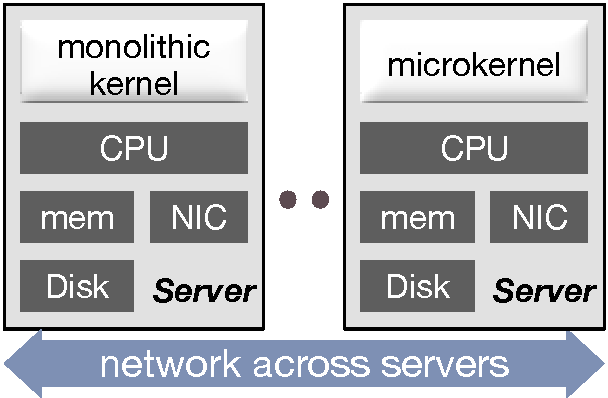
\includegraphics[width=1.7in]{lego/Figures/monolithic-arch.pdf}}
\caption[Monolithic OS.]{OSes Designed for Monolithic Servers.}
\label{fig-monolithic}
\end{center}
\end{subfigure}
\begin{minipage}{0.05in}
\hspace{0.05in}
\end{minipage}
\begin{subfigure}{1.8in}
\begin{center}
\centerline{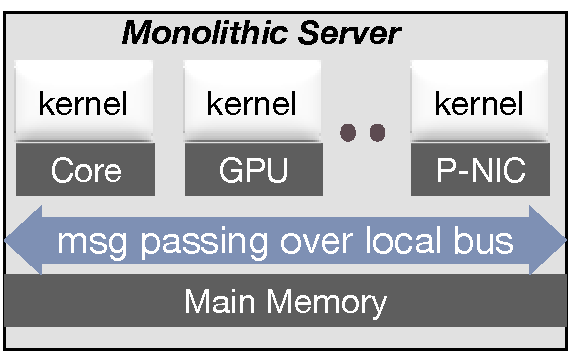
\includegraphics[width=1.8in]{lego/Figures/multikernel-arch.pdf}}
\caption[Multikernel Architecture.]{Multi-kernel Architecture. \small{P-NIC: programmable NIC.}}
\label{fig-multikernel}
\end{center}
\end{subfigure}
\begin{minipage}{0.05in}
\hspace{0.05in}
\end{minipage}
\begin{subfigure}{2.5in}
\begin{center}
\centerline{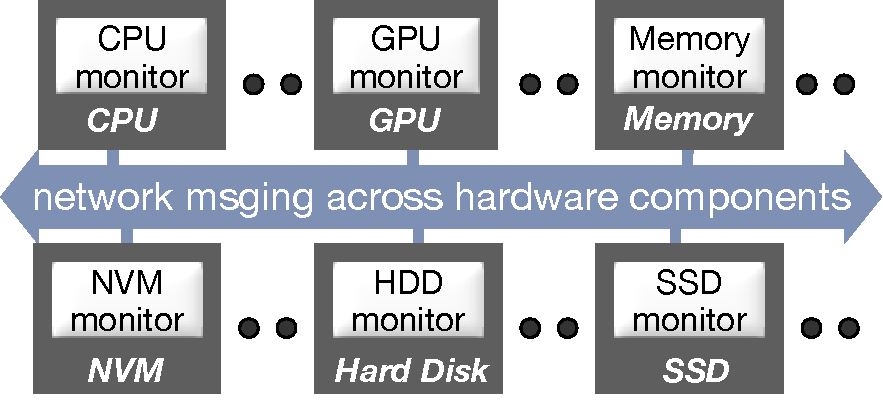
\includegraphics[width=2.6in]{lego/Figures/lego-arch.pdf}}
\caption[Splitkernel Architecture.]{Splitkernel Architecture.}
\label{fig-splitkernel}
\end{center}
\end{subfigure}
\caption[Operating System Architecture.]{Operating System Architecture.}
\end{figure*}
}

Another big challenge is to achieve scalability with only minimal hardware resources at \sysboard.
Our general idea is to avoid maintaining states or data structures that could grow with clients or \CN{}s.
For example, for \sys's memory system, we design the page table to have a total size proportional to the physical memory size on an \MN, 
not to the number of client processes using the \MN.
Similarly, we avoid maintaining any states that could grow with network flows or clients at \sysboard.
To achieve this while delivering end-to-end reliability, 
\sys\ 1) uses a connection-less, RPC-like interface, % on top of a standard Ethernet link layer,
2) treats network errors as \sys\ request failure and re-executes the entire request, 
3) shifts stateful tasks like re-execution, packet ordering, and congestion control to the \CN\ side, % (in \syslib\ software),
and 4) removes ordering guarantees from the network and provides memory operation ordering at \syslib.

The rest of the paper will dive deep into \sys\ design and our FPGA prototype implementation.
We built five applications on top of \sys:
an image compression utility, a binary-tree index, a key-value store, a multi-version object store, and a simple data analytics service.
%We prototyped \sys's memory device with FPGA (\sysboard).
%\sys\ achieves high throughput (100\Gbps\ with FPGA prototype), low (tail) latency (XXX\mus\ end-to-end MTU round trip latency), 
%low cost (XXX\x\ energy saving), %and great extendibility,
%and \sys\ scales well with XXX. %eliminates {\em all} scalability bottlenecks in both its memory and network systems.
We compared \sys\ with vanilla RDMA, two RDMA-based disaggregated/remote memory systems~\cite{Tsai20-ATC,Kalia14-RDMAKV}, 
%an FPGA-based RDMA implementation~\cite{StRoM}, 
and a software-based SmartNIC~\cite{BlueField}.
\sys\ scales much better and has orders of magnitude lower tail latency than RDMA, 
while achieving similar throughput and min latency as RDMA (even with the slower FPGA frequency in our prototype).
\sys\ has 1.1\x\ to 3.4\x\ energy saving compared to CPU-based and SmartNIC-based disaggregated memory systems 
and is 2.7\x\ faster than SmartNIC solutions. 

\fi
